\subsection{Geometry}
The $60$ kV geometry was derived from the technical drawings in \cite{espig}. Some simplifications were made especially regarding the inner part of the electrode, such that the geometry may be modeled as being rotationally symmetric. The dimensions of the electrode, puck, puck elevator, vacuum chamber and insulator were derived from Figure A.1, A.2, A.3, A.4 and A.6 in \cite{espig} respectively. The geometry of the vacuum chamber was also simplified to reduce the computational domain and the reduced insulator geometry is in part based on the drawing in Figure 5.7 of the thesis.
The boundary conditions were retrieved from Table 5.1 in \cite{espig} and the relative permittivity of the insulator was taken from an existing CST model to be $9.4$.

The geometry is depicted in fig.~\ref{fig:geometry} and a technical drawing of the actual geometry is given in fig.~\ref{fig:cad_geometry} for comparison. The numbers in the simplified geometry refer to the individual patches in the context of IGA. The patch boundaries are indicated by the black lines. The red lines represent homogeneous Dirichlet boundary conditions, the blue lines inhomogeneous Dirichlet boundary conditions with a value of $-60\ \mathrm{kV}$ and the green lines indicate homogeneous Neumann boundaries.
According to the technical drawings patch $10$ as well as parts of patches $7$ and $8$ are modeled as insulator material.

\begin{center}
\begin{figure}[H]
  \begin{tikzpicture}

\begin{axis}[
  enlargelimits=true,
  colormap/YlOrRd,
  point meta min = 0,
  point meta max = 5,
  x unit=m,
  y unit=m,
  legend pos=outer north east]

  \addplot[surf, shader=interp] table[point meta=\thisrow{c}]{figures/60kV/geometry/geometry_1.dat};

  \addplot[surf, shader=interp] table[point meta=\thisrow{c}]{figures/60kV/geometry/geometry_2.dat};

  \addplot[surf, shader=interp] table[point meta=\thisrow{c}]{figures/60kV/geometry/geometry_3.dat};

  \addplot[surf, shader=interp] table[point meta=\thisrow{c}]{figures/60kV/geometry/geometry_4.dat};

  \addplot[surf, shader=interp] table[point meta=\thisrow{c}]{figures/60kV/geometry/geometry_5.dat};

  \addplot[surf, shader=interp] table[point meta=\thisrow{c}]{figures/60kV/geometry/geometry_6.dat};

  \addplot[surf, shader=interp] table[point meta=\thisrow{c}]{figures/60kV/geometry/geometry_7.dat};

  \addplot[surf, shader=interp] table[point meta=\thisrow{c}]{figures/60kV/geometry/geometry_8.dat};

  \addplot[surf, shader=interp] table[point meta=\thisrow{c}]{figures/60kV/geometry/geometry_9.dat};

  \addplot[surf, shader=interp] table[point meta=\thisrow{c}]{figures/60kV/geometry/geometry_10.dat};

  \addplot[surf, shader=interp] table[point meta=\thisrow{c}]{figures/60kV/geometry/geometry_11.dat};

  \addplot[surf, shader=interp] table[point meta=\thisrow{c}]{figures/60kV/geometry/geometry_12.dat};

  \addplot[surf, shader=interp] table[point meta=\thisrow{c}]{figures/60kV/geometry/geometry_13.dat};

  /tikz/font=\normalfont\tiny
  % add patch indices
  \addplot[only marks, point meta=explicit symbolic, color=black, nodes near coords] coordinates{
  (0.14,-0.001) [(1)]
  (0.14,0.013) [(2)]
  (0.14,0.05) [(3)]
  (0.12,0.1) [(4)]
  (0.04,0.1) [(5)]
  (-0.025,0.06) [(6)]
  (-0.025,0.03) [(7)]
  (-0.021,0.02) [(8)]
  (-0.022,0.011) [(9)]
  (-0.025,0) [(10)]
  (0.016,0.012) [(11)]
  (0.027,0.017) [(12)]
  (0.055,0.021) [(13)]
  };

  % add patch boundaries
  \addplot[color=brewergreen, line width=1pt] table{figures/60kV/boundary/boundaries11.dat};
  \addplot[color=brewergrey] table{figures/60kV/boundary/boundaries12.dat};
  \addplot[color=brewerblue, line width=1pt] table{figures/60kV/boundary/boundaries13.dat};
  \addplot[color=brewerred, line width=1pt] table{figures/60kV/boundary/boundaries14.dat};

  \addplot[color=brewergrey] table{figures/60kV/boundary/boundaries21.dat};
  \addplot[color=brewergrey] table{figures/60kV/boundary/boundaries22.dat};
  \addplot[color=brewerblue, line width=1pt] table{figures/60kV/boundary/boundaries23.dat};
  \addplot[color=brewerred, line width=1pt] table{figures/60kV/boundary/boundaries24.dat};

  \addplot[color=brewergrey] table{figures/60kV/boundary/boundaries31.dat};
  \addplot[color=brewergrey] table{figures/60kV/boundary/boundaries32.dat};
  \addplot[color=brewerblue, line width=1pt] table{figures/60kV/boundary/boundaries33.dat};
  \addplot[color=brewerred, line width=1pt] table{figures/60kV/boundary/boundaries34.dat};

  \addplot[color=brewerblue, line width=1pt] table{figures/60kV/boundary/boundaries41.dat};
  \addplot[color=brewerred, line width=1pt] table{figures/60kV/boundary/boundaries42.dat};
  \addplot[color=brewergrey] table{figures/60kV/boundary/boundaries43.dat};
  \addplot[color=brewergrey] table{figures/60kV/boundary/boundaries44.dat};

  \addplot[color=brewerblue, line width=1pt] table{figures/60kV/boundary/boundaries51.dat};
  \addplot[color=brewerred, line width=1pt] table{figures/60kV/boundary/boundaries52.dat};
  \addplot[color=brewergrey] table{figures/60kV/boundary/boundaries53.dat};
  \addplot[color=brewergrey] table{figures/60kV/boundary/boundaries54.dat};

  \addplot[color=brewergrey] table{figures/60kV/boundary/boundaries61.dat};
  \addplot[color=brewergrey] table{figures/60kV/boundary/boundaries62.dat};
  \addplot[color=brewerred, line width=1pt] table{figures/60kV/boundary/boundaries63.dat};
  \addplot[color=brewerblue, line width=1pt] table{figures/60kV/boundary/boundaries64.dat};

  \addplot[color=brewergrey] table{figures/60kV/boundary/boundaries71.dat};
  \addplot[color=brewergrey] table{figures/60kV/boundary/boundaries72.dat};
  \addplot[color=brewerred, line width=1pt] table{figures/60kV/boundary/boundaries73.dat};
  \addplot[color=brewerblue, line width=1pt] table{figures/60kV/boundary/boundaries74.dat};

  \addplot[color=brewergrey] table{figures/60kV/boundary/boundaries81.dat};
  \addplot[color=brewergrey] table{figures/60kV/boundary/boundaries82.dat};
  \addplot[color=brewerred, line width=1pt] table{figures/60kV/boundary/boundaries83.dat};
  \addplot[color=brewerblue, line width=1pt] table{figures/60kV/boundary/boundaries84.dat};

  \addplot[color=brewergrey] table{figures/60kV/boundary/boundaries91.dat};
  \addplot[color=brewergrey] table{figures/60kV/boundary/boundaries92.dat};
  \addplot[color=brewerred, line width=1pt] table{figures/60kV/boundary/boundaries93.dat};
  \addplot[color=brewergrey] table{figures/60kV/boundary/boundaries94.dat};

  \addplot[color=brewergreen, line width=1pt] table{figures/60kV/boundary/boundaries101.dat};
  \addplot[color=brewergrey] table{figures/60kV/boundary/boundaries102.dat};
  \addplot[color=brewerred, line width=1pt] table{figures/60kV/boundary/boundaries103.dat};
  \addplot[color=brewerblue, line width=1pt] table{figures/60kV/boundary/boundaries104.dat};

  \addplot[color=brewerblue, line width=1pt] table{figures/60kV/boundary/boundaries111.dat};
  \addplot[color=brewerblue, line width=1pt] table{figures/60kV/boundary/boundaries112.dat};
  \addplot[color=brewergrey] table{figures/60kV/boundary/boundaries113.dat};
  \addplot[color=brewergrey] table{figures/60kV/boundary/boundaries114.dat};

  \addplot[color=brewergrey] table{figures/60kV/boundary/boundaries121.dat};
  \addplot[color=brewergrey] table{figures/60kV/boundary/boundaries122.dat};
  \addplot[color=brewerblue, line width=1pt] table{figures/60kV/boundary/boundaries123.dat};
  \addplot[color=brewerblue, line width=1pt] table{figures/60kV/boundary/boundaries124.dat};

  \addplot[color=brewerblue, line width=1pt] table{figures/60kV/boundary/boundaries131.dat};
  \addplot[color=brewerblue, line width=1pt] table{figures/60kV/boundary/boundaries132.dat};
  \addplot[color=brewergrey] table{figures/60kV/boundary/boundaries133.dat};
  \addplot[color=brewerblue, line width=1pt] table{figures/60kV/boundary/boundaries134.dat};

\end{axis}
\end{tikzpicture}

  \caption{60 kV Photocathode geometry and boundary conditions.}
  \label{fig:geometry}
\end{figure}
\end{center}

\begin{center}
\begin{figure}[H]
  \includegraphics[width=\textwidth]{figures/60kV/geometry}
  \caption{Part of the CAD drawing of the geometry.}
  \label{fig:cad_geometry}
\end{figure}
\end{center}

\subsection{Electrostatic Potential and Electric Field}
\label{sec:potential_field}
The solution for the electrostatic potential is shown in fig.~\ref{fig:potential}. Fig.~\ref{fig:electric_field} depicts the absolute value of the electric field.
Both of the solutions were computed with $p=4$ as the degree of the basis functions and $n_\mathrm{sub}=128$ as the number of elements that each knot vector is uniformly split into.
To give a comparison with the previous simulations fig.~\ref{fig:phd_electric_field} shows the results depicted in the thesis \cite{espig}. It is visible that the solutions are similar with the peak values appearing near the circular parts of the electrode. However the new results indicate that the absolute largest values occur at the back of the electrode and they also show higher field magnitudes in the insulator regions. This is a clear contrast to the previous simulation.
A second comparison can be made with the updated CST model from fig.~\ref{fig:electric_field_wende} from \cite{wende}. The absolute largest field values appear in the same region, however their magnitude is higher.
The bevavior of the field at the triple point is also very similar in that the surrounding magnitudes are very small.

\begin{center}
\begin{figure}[H]
  \includegraphics[width=\textwidth]{figures/60kV/potential}
  \caption{Electrostatic potential.}
  \label{fig:potential}
\end{figure}
\end{center}

\begin{center}
\begin{figure}[H]
  \includegraphics[width=\textwidth]{figures/60kV/gradient}
  \caption{Absolute value of the electric field.}
  \label{fig:electric_field}
\end{figure}
\end{center}

\begin{center}
\begin{figure}[H]
  \includegraphics[width=\textwidth]{figures/60kV/electric_field}
  \caption{Results from the PhD thesis.}
  \label{fig:phd_electric_field}
\end{figure}
\end{center}

\begin{center}
\begin{figure}[H]
  \includegraphics[width=\textwidth]{figures/60kV/electric_field_wende}
  \caption{Results from the Bachelor thesis.}
  \label{fig:electric_field_wende}
\end{figure}
\end{center}

\subsection{Convergence Study}
The convergence studies investigate the accuracy of the solution while increasing the number of elements per patch. (Akin to $h$-refinement in classical FEA) Since no analytic solution exists we used a reference with $n_\mathrm{sub}=256$ and $p=4$ as a comparison.
The errors are computed as
\begin{align}
  e_{L^2} = \frac{\| \varphi_\mathrm{it} - \varphi_\mathrm{ref} \|_{L^2}}{\| \varphi_\mathrm{ref} \|_{L^2}}\\
  e_{H^1} = \frac{\| \varphi_\mathrm{it} - \varphi_\mathrm{ref} \|_{H^1}}{\| \varphi_\mathrm{ref} \|_{H^1}}
\end{align}
where
\begin{align}
  \| \varphi \|_{H^1} = \sqrt{ \| \varphi \|_{L^2}^2 + \| \nabla\varphi \|_{L^2}^2 }.
\end{align}
Here $\varphi$ denotes the electrostatic potential. The integrals associated with the $L^2$-norm are evaluated using a quadrature rule defined on each element of a given patch.

The degrees of the basis functions are given in the legend, as well as theoretical limits for the convergence rates. They are given by $p+1$ in the case of the $L^2$-norm (electrostatic potential) and $p$ in the case of the $H^1$-norm (electric field). As seen in fig.~\ref{fig:convergence_potential} and fig.~\ref{fig:convergence_gradient} we observe convergence, however the convergence rate appears to be limited.

\begin{figure}[H]
  \begin{center}
    \begin{tikzpicture}

\begin{loglogaxis}[
  xlabel={$1/nsub$},
  ylabel={relative error},
  legend entries={$p=2$, $h^{2+1}$, $p=3$, $h^{3+1}$, $p=4$, $h^{4+1}$},
  legend pos=outer north east]

\addplot [color=brewerred] table[x=h, y=errl2]{figures/insulator/convergence/convergence_ref=5_degree=2.dat};

\addplot [color=brewergrey] table[x=h, y=h_l2]{figures/insulator/convergence/convergence_ref=5_degree=2.dat};

\addplot [color=brewerblue] table[x=h, y=errl2]{figures/insulator/convergence/convergence_ref=5_degree=3.dat};

\addplot [color=brewergrey] table[x=h, y=h_l2]{figures/insulator/convergence/convergence_ref=5_degree=3.dat};

\addplot [color=brewergreen] table[x=h, y=errl2]{figures/insulator/convergence/convergence_ref=5_degree=4.dat};

\addplot [color=brewergrey] table[x=h, y=h_l2]{figures/insulator/convergence/convergence_ref=5_degree=4.dat};

\end{loglogaxis}
\end{tikzpicture}

    \caption{Convergence of $L^2$-norm.}
    \label{fig:convergence_potential}
  \end{center}
\end{figure}

\begin{figure}[H]
  \begin{center}
    \begin{tikzpicture}

\begin{loglogaxis}[
  xlabel={$1/nsub$},
  ylabel={relative error},
  legend entries={$p=2$, $h^{2}$, $p=3$, $h^{3}$, $p=4$, $h^{4}$},
  legend pos=outer north east]

\addplot [color=brewerred] table[x=h, y=errh1]{figures/insulator/convergence/convergence_ref=5_degree=2.dat};

\addplot [color=brewergrey] table[x=h, y=h_h1]{figures/insulator/convergence/convergence_ref=5_degree=2.dat};

\addplot [color=brewerblue] table[x=h, y=errh1]{figures/insulator/convergence/convergence_ref=5_degree=3.dat};

\addplot [color=brewergrey] table[x=h, y=h_h1]{figures/insulator/convergence/convergence_ref=5_degree=3.dat};

\addplot [color=brewergreen] table[x=h, y=errh1]{figures/insulator/convergence/convergence_ref=5_degree=4.dat};

\addplot [color=brewergrey] table[x=h, y=h_h1]{figures/insulator/convergence/convergence_ref=5_degree=4.dat};

\end{loglogaxis}
\end{tikzpicture}

    \caption{Convergence of $H^1$-norm.}
    \label{fig:convergence_gradient}
  \end{center}
\end{figure}

Lastly the error in specific regions of the geometry was investigated by displaying the absolute error of the eletric field on every individual element of the mesh. In the case of fig.~\ref{fig:error_elem} we chose $n_\mathrm{sub}=256$ and $p=3$ for the iterative solution and computed the errors with respect to a reference using $n_\mathrm{sub}=256$ and $p=4$.
The figure shows the absolute error on each element in a logarithmic scale. We observe that the errors are largest near sharp corners or large changes in the sizes of the mesh's elements. This is to be expected and as indicated by the colorbar the largest absolute errors come out to be around $19\ \mathrm{V/m}$ with the associated field magnitudes being almost exclusively larger than $10\ \mathrm{MV/m}$.

\begin{center}
\begin{figure}[H]
  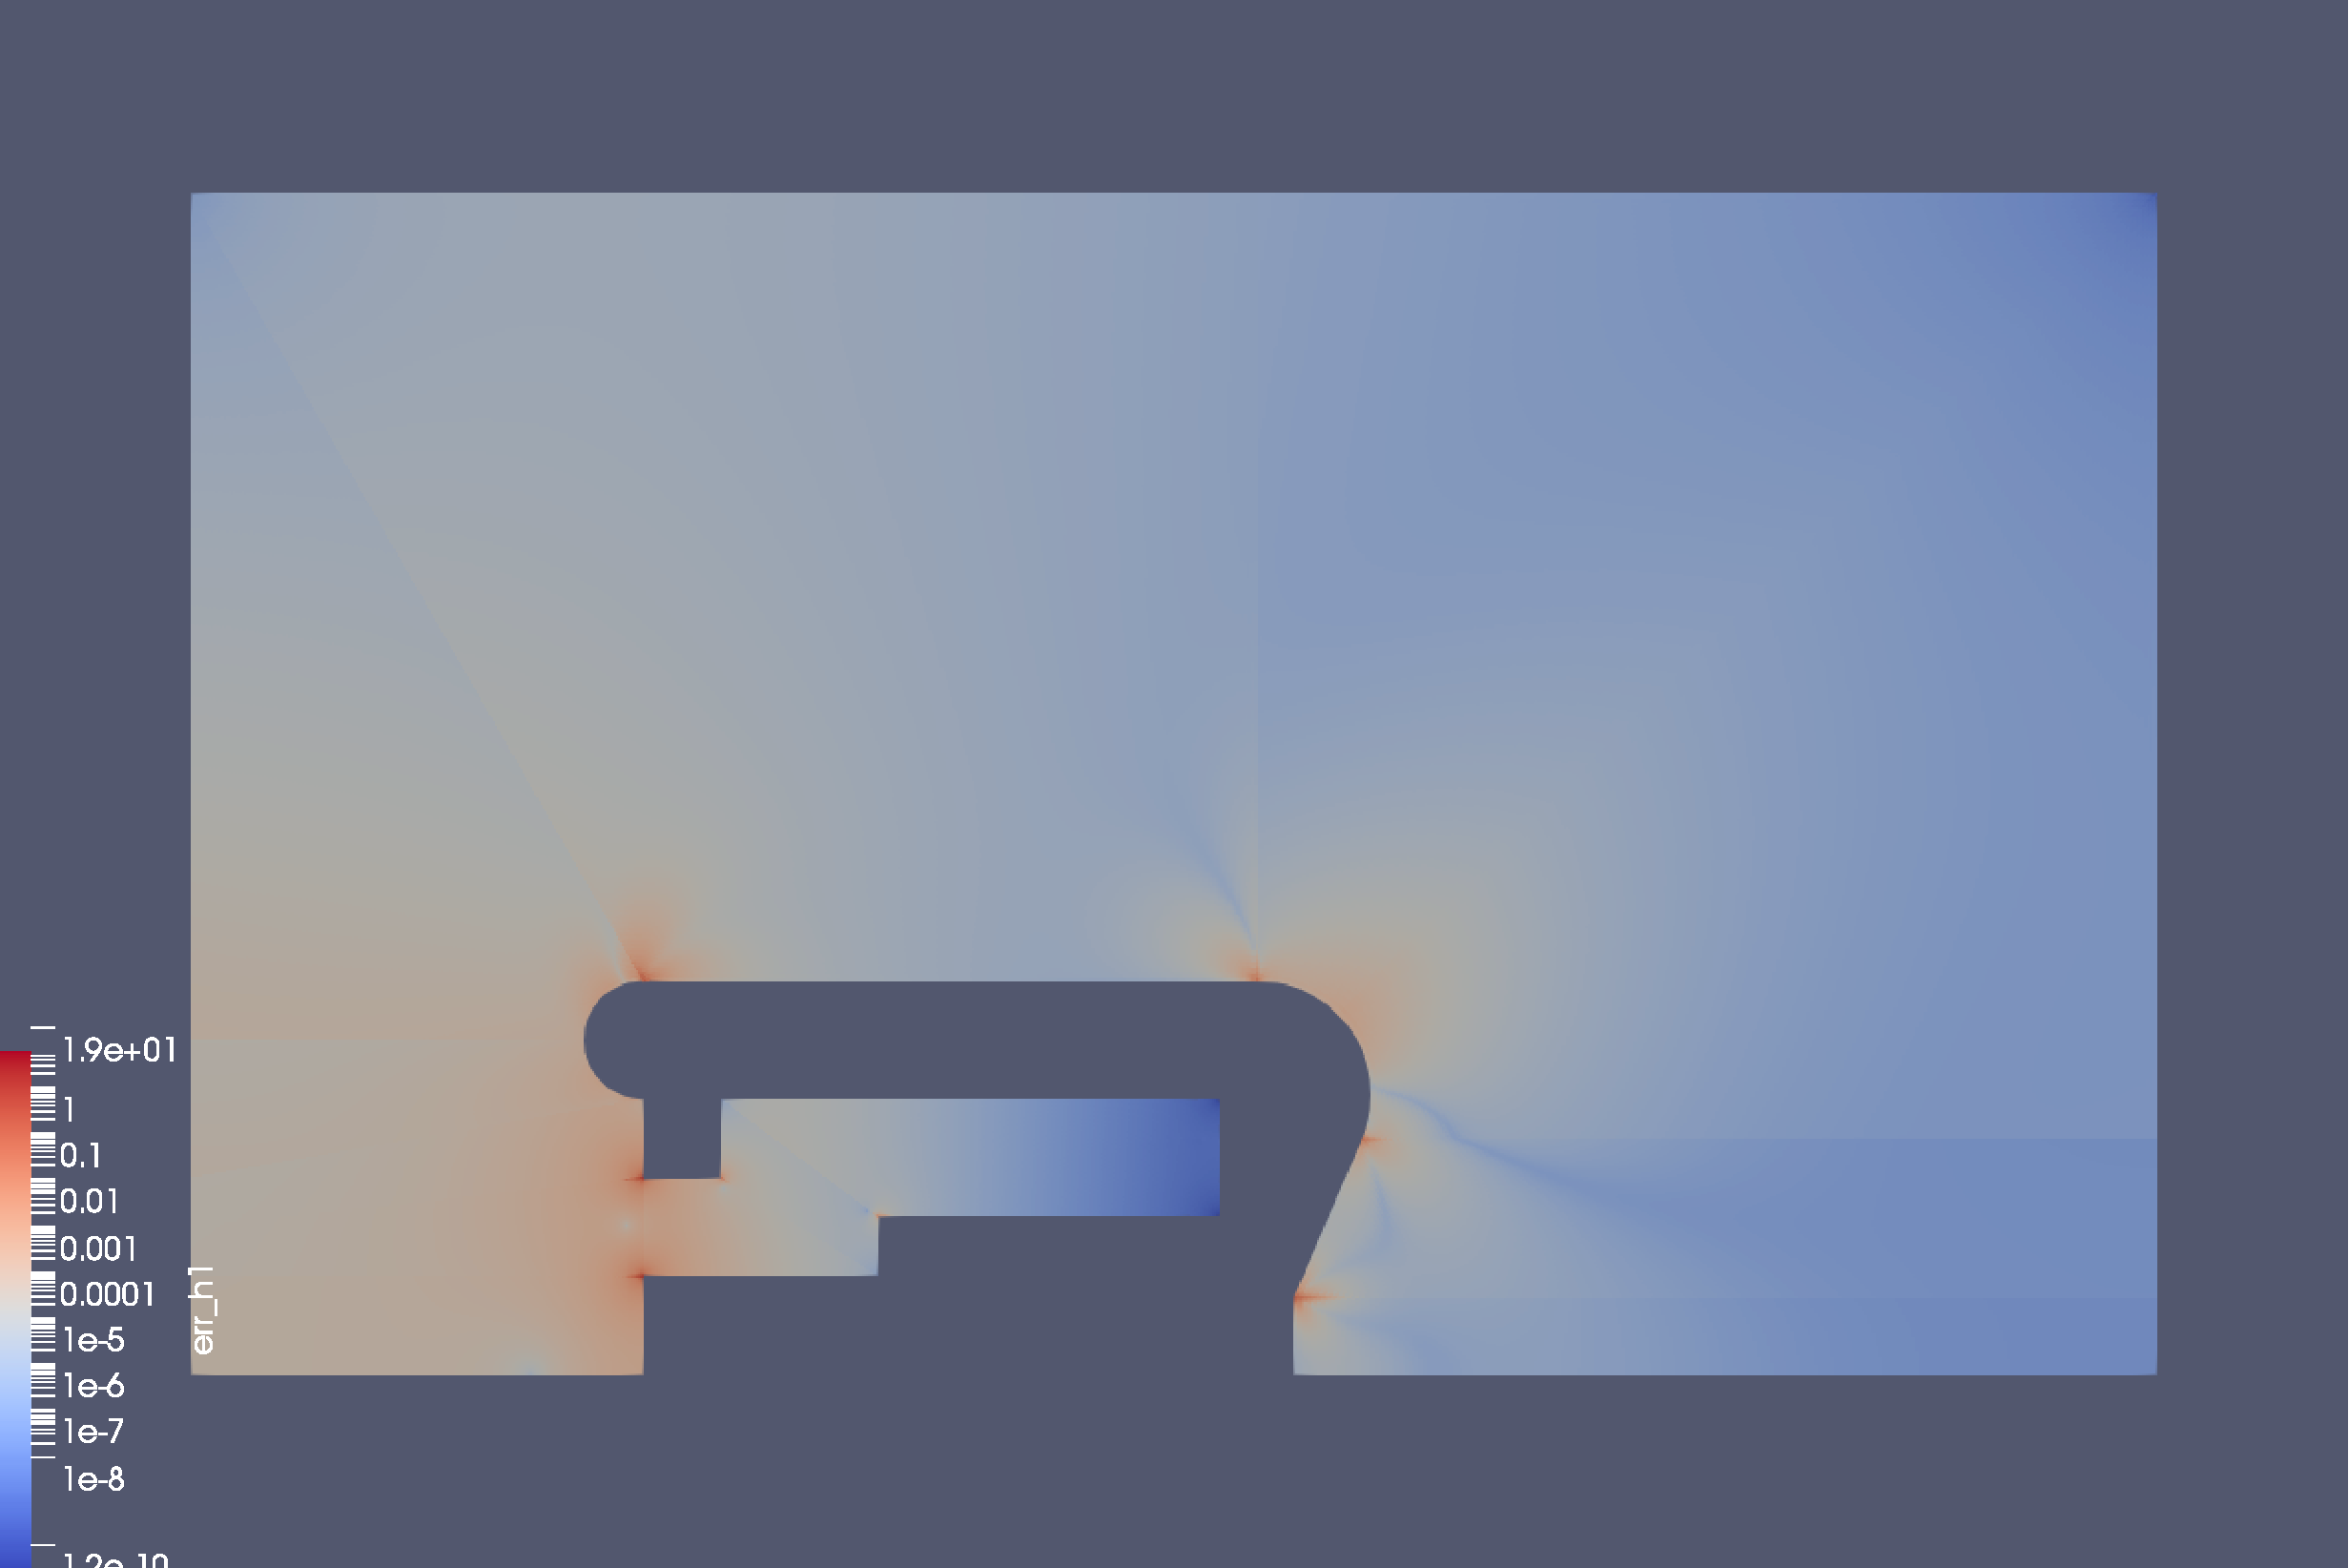
\includegraphics[width=\textwidth]{figures/60kV/error_elem}
  \caption{Absolute error of the electric field on every element.}
  \label{fig:error_elem}
\end{figure}
\end{center}
